 \section{ANTENNA CHARACTERISTICS}
 \subsection{Task description}
This task investigates a $5^{th}$ order, clock tuneable, switched capacitor filter and analysis of it's measurement results. Following were the main sub-objectives:
    \begin{itemize}
    \item Building of the SC filter using a LT1063 (dual ±5V supply), and tuning of the same with two clock frequencies (1\,MHz and 500\,kHz).
    \item Building of a non-inverting LM4562 preamplifier stage (gain = 100) in front of the SC filter.
    \item Measurement of the magnitude responses at both tuning frequencies.
    \item Investigation of the filter's behaviour when the input frequency approaches the tuning frequency.
    \item Investigation of the switching frequency visibility when applying a sine wave.
    \item Measurement of the total output noise using additional inverting amplifier stages (with LM4562).
    \item Determination of the total input noise voltage and the noise voltage density after setting Rg = 51Ω, and Rg = 100kΩ.
    \item Calculation of the SNR and ENOB on the SC-filter output for a full-scale sine wave.
    \end{itemize}
\subsection{Schematics}
Figure~\ref{fig:circuit_3} shows the schematic of the switched capacitor filter. The pre-amplifier stage is represented with a non-inverting amplifier circuit with AD823 OpAmp (Gain=100) but the actual pre-amplification was done with a non-inverting amplifier circuit with LM4562 OpAmp (Gain=100) as per the laboratory script.
\begin{figure}[ht!]
    \centering
    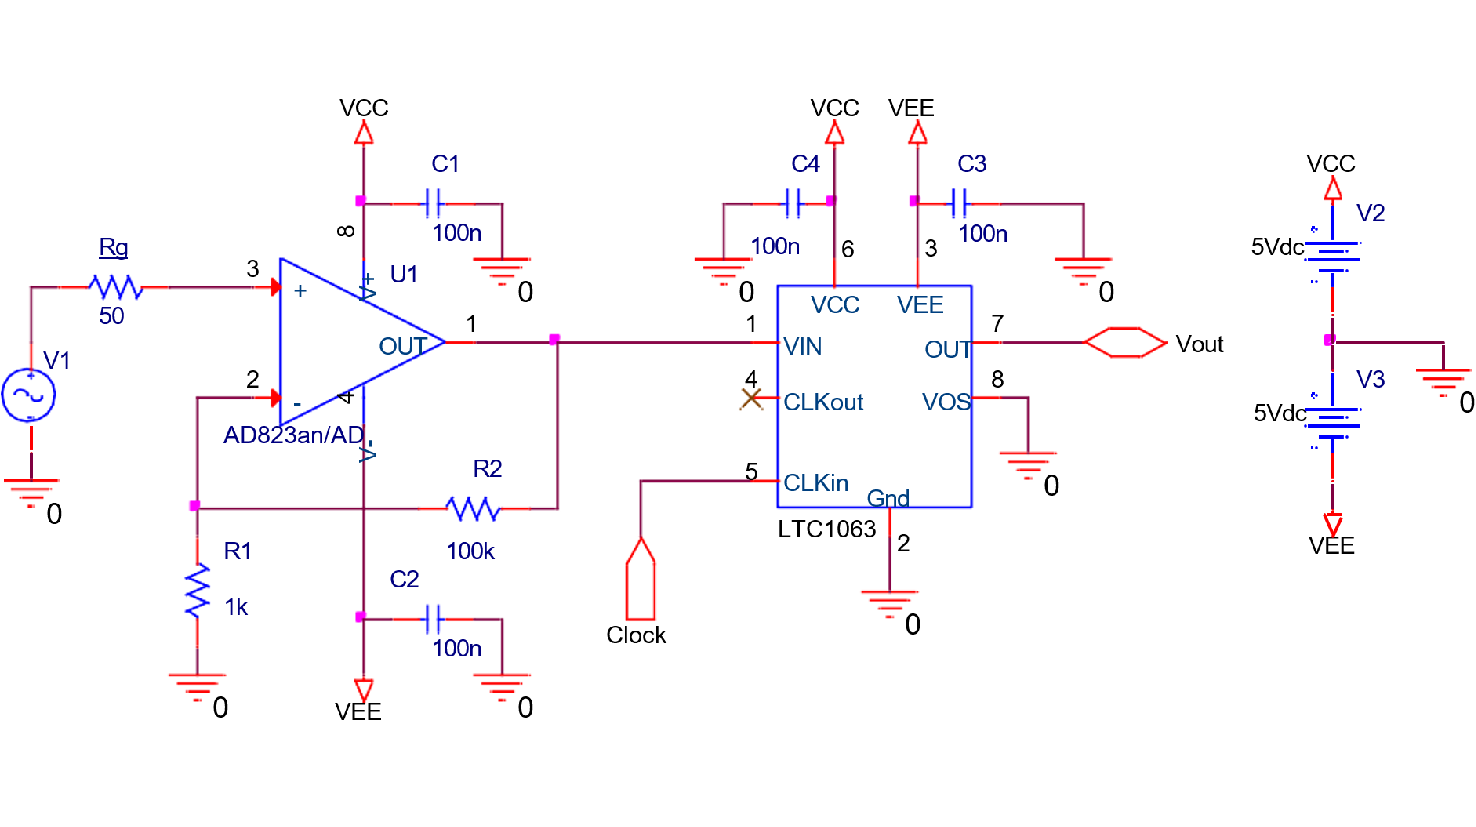
\includegraphics[page=1,width=0.7\linewidth]{src/diagrams/4_Switched-capacitors.pdf}
    \caption[\centering Schematic of the switched capacitor filter with pre-amplifier stage with LM4562] {\centering Schematic of the switched capacitor filter with pre-amplifier stage made of AD823 \cite{Amp}.}
    \label{fig:circuit_3}
\end{figure}
\newpage
Figure~\ref{fig:circuit_4} shows the schematic of the two additional inverting amplifier (LM4562) stages, connected to the output of the SC-filter circuit (second stage gain = -100, dual supply = ±5V, and SC-filter tuning frequency = 1MHz).
\begin{figure}[ht!]
    \centering
    \includegraphics[page=2,width=1.0\linewidth]{src/diagrams/4_Switched-capacitors.pdf}
    \caption{\centering Schematic of the two-stage inverting amplifiers for RMS noise measurement.}
    \label{fig:circuit_4}
\end{figure}
\subsection{Formulas and Calculations}
The following formulae (\ref{eq:23}) and (\ref{eq:24}) were used to calculate the SNR and ENOB. \cite{ACD}. \\
\begin{gather}
    SNR = 20log_{10}\Biggl(\frac{U_{in}Gain}{\sqrt{2}U_n}\Biggr)=49.40dB \label{eq:23}
 \end{gather}
\begin{gather}
    ENOB = \frac{SNR-1.76}{6.02}=7.914=8Bit \label{eq:24}
\end{gather}
\newpage
\subsection{Tables with measurement results}
Table \ref{tab:Bauteile3} shows the calculated, measured and selected component values for the switched capacitor filter. \\

\begin{table}[ht!]
\centering
\begin{tabular}{|c|c||c||c|}
	\hline
	Components & Selected & Measured & Calculated \\
    Resistors/Capacitors & $k\Omega / nF $ & $k\Omega / nF $ & $k\Omega / nF $\\\hline\hline
	$R_g$ & 0.05 & 0.051 & - \\
	\hline
    $R_1$ & 1 & 0.997 & - \\
	\hline
	  $R_2$ & 100 & 100.7 & - \\
	\hline
	$R_3$ & 0.91 & 0.908 & 0.851 \\
	\hline
	$R_4$ & 9.1 & 9.04 & 8.519 \\
	\hline
	$R_5$ & 2.7 & 2.69 & 2.635 \\
	\hline
	$R_6$ & 1 & 0.995 & - \\
	\hline
    $R_7$ & 100 & 100.7 & - \\
	\hline
	$C_1$ & 100 & 99 & - \\
	\hline
	$C_2$ & 100 & 100 & - \\
	\hline
	$C_3$ & 100 & 103 & - \\
	\hline
	$C_4$ & 100 & 103 & - \\
	\hline
    $C_5$ & 0.15 & 0.198 & - \\
	\hline
    $C_6$ & 4.7 & 4.69 & - \\
	\hline
    $C_7$ & 1500 & 1501 & 1863 \\
	\hline
    $C_8$ & 100 & 100.09 & - \\
	\hline
    $C_9$ & 10000 & 10030 & - \\
	\hline
	$C_{10}$ & 100 & 101 & - \\
	\hline
	$C_{11}$ & 10000 & 9950 & - \\
	\hline
\end{tabular}
\caption{\centering Measured values for the resistors and capacitors use for the switched capacitor filter, the pre-amplification stage, and the two inverting amplifier stages.}
\label{tab:Bauteile3}
\end{table}
% Table generated by Excel2LaTeX from sheet 'Tabelle2'

\begin{table}[ht!]
\centering
\begin{tabular}{|c||c|}
    \hline
    \textbf{Adjusted} &
    \textbf{Measured} \\
    \hline
    $R_g$ / $\Omega$ & $U_n$ / mV \\
    \hline\hline
    51 & 125.16 \\
    100k & 239.3 \\
    \hline
    \end{tabular}
    \caption{\centering Measured values for total noise voltage of the switched capacitor filter for 2 values of $R_g$.}
    \label{tab:mes}
\end{table}

\newpage
\subsection{Measurement curves and diagrams}
Figure~\ref{fig:bode3} shows the bode plot of the switched capacitor filter, along with the pre-amplification stage. Gain of the circuit at frequency values of 500kHz and 1MHz are illustrated here. \\
Tables \ref{tab:Messermunt_4} and \ref{tab:Messermunt_3} show the measured Gain values for both tuning frequencies. 
\begin{figure}[ht!]
    \centering
    \includegraphics[page=12,width=0.8\linewidth]{src/diagrams/4_Switched-capacitors.pdf}
    \caption{\centering Magnitude response of the switched capacitor filter ($U_{in}$=20mVpp).}
    \label{fig:bode3}
\end{figure}
\FloatBarrier
Figure~\ref{fig:22} shows the output waveform of the switched capacitor filter along with the pre-amplification stage. The input frequency is set near tuning frequency.
\begin{figure}[ht!]
    \centering
    \includegraphics[page=3,width=0.9\linewidth]{src/diagrams/4_Switched-capacitors.pdf}
    \caption{\centering Output plot of the switched capacitor filter ($U_{in}$=20mVpp, $f$=998kHz)}
    \label{fig:22}
\end{figure}
\newpage
Figure~\ref{fig:23} shows the output voltage corresponding to a sine wave as input voltage. Once zoomed in, the switching frequency is visible in the output voltage characterized by the step-like appearance. 
\begin{figure}[ht!]
    \centering
    \includegraphics[page=6,width=0.9\linewidth]{src/diagrams/4_Switched-capacitors.pdf}
    \caption{\centering Resultant waveform depicting the switching frequency ($U_{in}$=20mVpp, $f$=5kHz)}
    \label{fig:23}
\end{figure}
\FloatBarrier
Figure~\ref{fig:24} shows the measurement of the total noise voltage at the output of the filter including the inverting amplifier stages. The readings are illustrated using the RMS function as recommended.  
\begin{figure}[ht!]
    \centering
    \includegraphics[page=8,width=0.9\linewidth]{src/diagrams/4_Switched-capacitors.pdf}
    \caption{\centering Resultant graph showing the output noise with $R_g$=100k$\Omega$.}
    \label{fig:24}
\end{figure}
\subsection{Discussion}
\begin{itemize}
    \item Figure~\ref{fig:bode3} shows the Bode plot of the SC filter. Two different tuning frequencies were used for the measurements 500\,kHz and 1\,MHz. As expected for a switched capacitor filter, the lower the clock frequency, the attenuation begins at a lower cut-off frequency. 
    \item Figure~\ref{fig:22} shows the output voltage when the tuning frequency is close to the input frequency. 
    \item Figure~\ref{fig:23} shows a sine wave with $\hat{u}$=20mVpp and $f$=998kHz as the input signal. It can be seen that the output is an amplified sine wave with a frequency of 1.996\,kHz. This frequency is the difference between the set input frequency and the clock frequency (1MHz). When the input is close to the clock frequency, sampling creates a low “difference” (alias/beat) frequency in the output.
    \item Figure~\ref{fig:24} depicts the noise measurement using the RMS function.
    \item The SNR and ENOB values were also calculated (see \ref{eq:23} and \ref{eq:24}).
\end{itemize}
